\begin{tikzpicture}[foundation picture,font=\figurefont\fontsize{8.5}{11}\selectfont]
\path[use as bounding box] (0,-5) rectangle(169,101);
\node[inner sep=0pt] at (34,49) {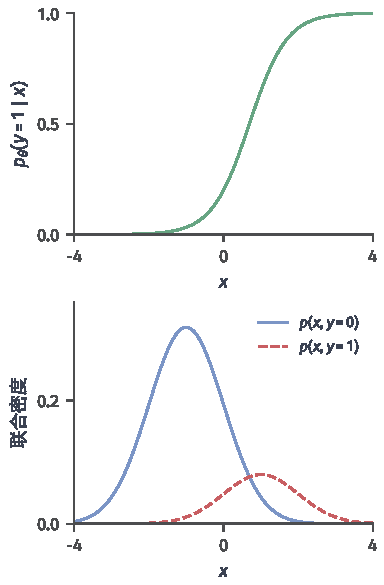
\includegraphics[width=65mm]{figures/02-foundations/01-basics/tikz/models-discriminative-generative/models-discriminative-generative.pdf}};
\node[anchor=west] at (72,96) {判别式：直接估计};
\node[foundation model,minimum width=28mm] (s) at (84,75) {$s=f_\theta(\bm x)$\\$s=\ln3$};
\node[foundation model,minimum width=17mm] (sig) at (119,75) {$\sigma(s)$};
\node[foundation output,minimum width=28mm] (o) at (153,75) {$p_1=0.75$\\$p_0=0.25$};
\draw[foundation flow] (s)--(sig);\draw[foundation flow] (sig)--(o);
\node[anchor=west] at (72,47) {生成式：联合概率再归一化};
\node[foundation node,fill=FigureRedFill,minimum width=39mm] (j1) at (91,30) {$y=1$：$0.2\times0.12=0.024$};
\node[foundation node,fill=FigureBlueFill,minimum width=39mm] (j0) at (91,10) {$y=0$：$0.8\times0.01=0.008$};
\node[foundation model,minimum width=15mm] (n) at (126,20) {$\div0.032$};
\node[foundation output,minimum width=24mm] (g) at (156,20) {$p_1=0.75$\\$p_0=0.25$};
\draw[foundation flow] (j1.east)--(115,30)--(n.north);\draw[foundation flow] (j0.east)--(115,10)--(n.south);\draw[foundation flow] (n)--(g);
\end{tikzpicture}